% Adjust these for the path of the theme and its graphics, relative to this file
%\usepackage{beamerthemeFalmouthGamesAcademy}
\usepackage{../../beamerthemeFalmouthGamesAcademy}
\usepackage{multimedia}
\graphicspath{ {../../} }

% Default language for code listings
\lstset{language=Python
}

% For strikethrough effect
\usepackage[normalem]{ulem}
\usepackage{wasysym}

\usepackage{pdfpages}

% http://www.texample.net/tikz/examples/state-machine/
\usetikzlibrary{arrows,automata}

\newcommand{\modulecode}{COMP140 GAM160}\newcommand{\moduletitle}{Hacking Hardware/Advanced Programming}\newcommand{\sessionnumber}{Session 6}

\begin{document}
\title{\sessionnumber: Basic Principles for Computation}
\subtitle{\modulecode: \moduletitle}

\frame{\titlepage} 

\part{Worksheet 1}
\frame{\partpage}

\begin{frame}{Worksheet 1}
    \begin{itemize}
        \item Due \textbf{tomorrow}!
        \item Support workshop \textbf{later this afternoon}
    \end{itemize}
\end{frame}

\begin{frame}{Worksheet submission}
    \begin{itemize}
        \item \url{https://github.com/falmouth-games-academy/comp110-worksheet-1}
        \item If the YouTube uploader within SpaceChem does not work,
            save the video to disk and upload to YouTube manually
        \item If this also doesn't work, use e.g.\ OBS to record videos and upload them
            (I only need to see your solutions running)
        \item If \textbf{this} doesn't work, record your screen with your phone!
    \end{itemize}
\end{frame}

\begin{frame}{Worksheet submission}
    \begin{itemize}
        \item \url{https://github.com/falmouth-games-academy/comp110-worksheet-1}
        \item Don't forget to upload your \textbf{save file}, add your \textbf{playlist link}, and open a \textbf{pull request}
        \item Please make sure I can figure out who you are!
            If it's not obvious from your username, please put your \textbf{name or student number}
            in the title of your pull request
        \item Any problems, send me a message via email or slack
    \end{itemize}
\end{frame}

\part{Binary notation}
\frame{\partpage}

\begin{frame}
	\centering
	\includegraphics[width=0.7\textwidth]{10-types-of-people}
	\par\vspace{2ex}\par
	{\tiny Image credit: \url{http://www.toothpastefordinner.com}}
\end{frame}



\begin{frame}{How we write numbers}
	\begin{itemize}
		\pause\item We write numbers in \textbf{base~10}
		\pause\item We have 10 \textbf{digits}: $0, 1, 2, \dots, 8, 9$
		\pause\item When we write $6397$, we mean:
			\begin{itemize}
				\pause\item Six thousand, three hundred and ninety seven
				\pause\item (Six thousands) and (three hundreds) and (nine tens) and (seven)
				\pause\item $(6 \times 1000) + (3 \times 100) + (9 \times 10) + (7)$
				\pause\item $\left(6 \times 10^3\right)
				+ \left(3 \times 10^2\right)
				+ \left(9 \times 10^1\right)
				+ \left(7 \times 10^0\right)$
				\pause\item
				    \begin{tabular}{cccc}
				        Thousands & Hundreds & Tens & Units \\
				        6 & 3 & 9 & 7
				    \end{tabular}
			\end{itemize}
	\end{itemize}
\end{frame}

\begin{frame}{Binary}
	\begin{itemize}
		\pause\item Binary notation works the same, but is \textbf{base~2} instead of \textbf{base~10}
		\pause\item We have 2 \textbf{digits}: $0, 1$
		\pause\item When we write $10001011$ in binary, we mean: \par\pause
			$\phantom{+} \left(1 \times 2^7\right) + 
			\left(0 \times 2^6\right) + 
			\left(0 \times 2^5\right) + 
			\left(0 \times 2^4\right)$ \par
			$+ \left(1 \times 2^3\right) + 
			\left(0 \times 2^2\right) + 
			\left(1 \times 2^1\right) + 
			\left(1 \times 2^0\right)$ \par\pause
			$= 2^7 + 2^3 + 2^1 + 2^0$ \par\pause
			$= 128 + 8 + 2 + 1 \text{ (base 10)}$ \par\pause
			$= 139 \text{ (base 10)}$
	\end{itemize}
\end{frame}

\begin{frame}{Converting to binary}
    \begin{center}
        \url{https://www.youtube.com/watch?v=OezK_zTyvAQ}
    \end{center}
\end{frame}

\begin{frame}{Bits, bytes and words}
	\begin{itemize}
		\pause\item A \textbf{bit} is a \uline{b}inary dig\uline{it}
			\begin{itemize}
				\pause\item Can store a 0 or 1 (i.e.\ a boolean value)
			\end{itemize}
		\pause\item A \textbf{byte} is 8 \textbf{bits}
			\begin{itemize}
				\pause\item Can store a number between 0 and 255 in binary
			\end{itemize}
		\pause\item A \textbf{word} is the number of bits that the CPU works with at once
			\begin{itemize}
				\pause\item 32-bit CPU: 32 bits = 1 word
				\pause\item 64-bit CPU: 64 bits = 1 word
			\end{itemize}
		\pause\item An $n$-bit word can store a number between 0 and $2^{n} - 1$
			\begin{itemize}
				\pause\item $2^{16}-1 = 65,535$
				\pause\item $2^{32}-1 = 4,294,967,295$
				\pause\item $2^{64}-1 = 18,446,744,073,709,551,615$
			\end{itemize}
	\end{itemize}
\end{frame}

\newcommand{\carry}[1]{\uncover<#1->{$_1$}}
\newcommand{\nocarry}[1]{\phantom{$_1$}}

\begin{frame}{Addition with carry}
	In base 10:
	\begin{center}
		\begin{tabular}{lllll}
			& 1 & 2 & 3 & 4 \\
			+ & 5\nocarry{4} & 6\carry{3} & 7\carry{2} & 8\nocarry{1} \\\hline
			& \uncover<5->{6} & \uncover<4->{9} & \uncover<3->{1} & \uncover<2->{2}
		\end{tabular}
	\end{center}
\end{frame}

\begin{frame}{Addition with carry}
	In base 2:
	\begin{center}
		\fbox{$1 + 1 = 10$ \qquad $1 + 1 + 1 = 11$}
		
		\vspace{2ex}
		
		\begin{tabular}{lllllllll}
			& 0 & 1 & 1 & 0 & 1 & 1 & 1 & 0 \\
			+ &
				0\carry{8} &
				0\carry{7} &
				1\nocarry{6} &
				0\carry{5} &
				0\carry{4} &
				1\carry{3} &
				1\nocarry{2} &
				1 \\\hline
			&
				\uncover<9->{1} &
				\uncover<8->{0} &
				\uncover<7->{0} &
				\uncover<6->{1} &
				\uncover<5->{0} &
				\uncover<4->{1} &
				\uncover<3->{0} &
				\uncover<2->{1}
		\end{tabular}
	\end{center}
\end{frame}

\begin{frame}{Modular arithmetic}
    \begin{columns}
        \begin{column}{0.4\textwidth}
            \begin{center}
                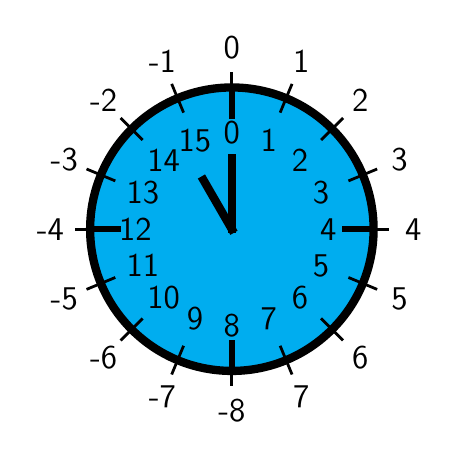
\begin{tikzpicture}[line cap=rect,line width=3pt,scale=0.9]
                    \filldraw [fill=cyan] (0,0) circle [radius=2cm];
                    \foreach \angle [count=\xi from 0] in {90,67.5,...,-247.5}
                    {
                        \draw[line width=1pt] (\angle:1.8cm) -- (\angle:2.2cm);
                        \node[font=\large] at (\angle:1.36cm) {\textsf{\xi}};
                    }
                    \foreach \angle [count=\xi from -8] in {270,247.5,...,-67.5}
                    {
                        \node[font=\large] at (\angle:2.56cm) {\textsf{\xi}};
                    }
                    \foreach \angle in {0,90,180,270}
                        \draw[line width=2pt] (\angle:1.6cm) -- (\angle:2cm);
                    \draw (0,0) -- (120:0.8cm);
                    \draw (0,0) -- (90:1cm);
                \end{tikzpicture}
            \end{center}
        \end{column}
        \begin{column}{0.55\textwidth}
            \begin{itemize}
                \pause\item Arithmetic \textbf{modulo} $N$
                \pause\item Numbers ``wrap around'' between $0$ and $N-1$
                \pause\item E.g.\ modulo $16$:
                    \begin{itemize}
                        \pause\item $14 + 7 = 5$
                        \pause\item $4 - 7 = 13$
                    \end{itemize}
            \end{itemize}
        \end{column}
    \end{columns}
\end{frame}

\begin{frame}{2's complement}
    \begin{itemize}
        \pause\item How can we represent negative numbers in binary?
        \pause\item Represent them modulo $2^n$ (for $n$ bits)
        \pause\item I.e.\ represent $-a$ as $2^n-a$
        \pause\item Instead of an $n$-bit number ranging from $0$ to $2^n-1$, it ranges from $-2^{n-1}$ to $+2^{n-1}-1$
        \pause\item E.g.\ 16-bit number ranges from $-32768$ to $+32767$
        \pause\item Note that the left-most bit can be interpreted as a \textbf{sign} bit:
            $1$ if negative, $0$ if positive or zero
    \end{itemize}
\end{frame}

\begin{frame}{Converting to 2's complement}
    \begin{itemize}
        \pause\item Convert the absolute value to binary
        \pause\item Invert all the bits (i.e.\ change $0 \leftrightarrow 1$)
        \pause\item Add 1
        \pause\item (This is equivalent to subtracting the number from $2^n$... why?)
        \pause\item This is also the process for converting back from 2's complement,
            i.e.\ doing it twice should give the original number
    \end{itemize}
\end{frame}

\begin{frame}{Why 2's complement?}
    \begin{itemize}
        \pause\item Allows all addition and subtraction to be carried out modulo $2^n$
            without caring whether numbers are positive or negative
        \pause\item In fact, subtraction can just be done as addition
        \pause\item I.e.\ $a-b$ is the same as $a+(-b)$, where $a$ and $-b$ are just $n$-bit numbers
    \end{itemize}
\end{frame}


\part{2's Complement}
\frame{\partpage}

\begin{frame}{Modular arithmetic}
    \begin{columns}
        \begin{column}{0.4\textwidth}
            \begin{center}
                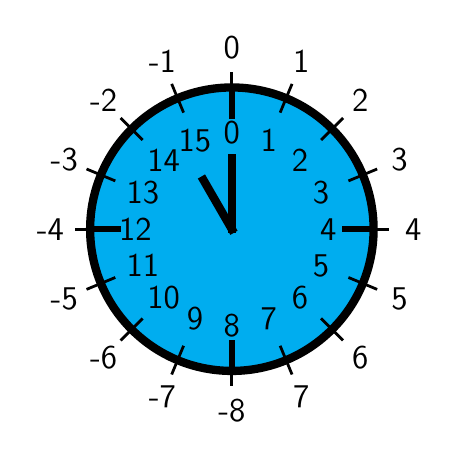
\begin{tikzpicture}[line cap=rect,line width=3pt,scale=0.9]
                    \filldraw [fill=cyan] (0,0) circle [radius=2cm];
                    \foreach \angle [count=\xi from 0] in {90,67.5,...,-247.5}
                    {
                        \draw[line width=1pt] (\angle:1.8cm) -- (\angle:2.2cm);
                        \node[font=\large] at (\angle:1.36cm) {\textsf{\xi}};
                    }
                    \foreach \angle [count=\xi from -8] in {270,247.5,...,-67.5}
                    {
                        \node[font=\large] at (\angle:2.56cm) {\textsf{\xi}};
                    }
                    \foreach \angle in {0,90,180,270}
                        \draw[line width=2pt] (\angle:1.6cm) -- (\angle:2cm);
                    \draw (0,0) -- (120:0.8cm);
                    \draw (0,0) -- (90:1cm);
                \end{tikzpicture}
            \end{center}
        \end{column}
        \begin{column}{0.55\textwidth}
            \begin{itemize}
                \pause\item Arithmetic \textbf{modulo} $N$
                \pause\item Numbers ``wrap around'' between $0$ and $N-1$
                \pause\item E.g.\ modulo $16$:
                    \begin{itemize}
                        \pause\item $14 + 7 = 5$
                        \pause\item $4 - 7 = 13$
                    \end{itemize}
            \end{itemize}
        \end{column}
    \end{columns}
\end{frame}

\begin{frame}{Modulo operator}
    \begin{itemize}
        \pause\item Present in many programming languages (including C++, C\#, Python) as \lstinline{\%}
        \pause\item \lstinline{a \% b} gives the \textbf{remainder} of \lstinline{a} divided by \lstinline{b}
        \pause\item E.g.\ \lstinline{21 \% 16} gives 5
        \pause\item Useful for wrapping around e.g.\ loop indexes or screen coordinates
    \end{itemize}
\end{frame}

\begin{frame}{2's complement}
    \begin{itemize}
        \pause\item How can we represent negative numbers in binary?
        \pause\item Represent them modulo $2^n$ (for $n$ bits)
        \pause\item I.e.\ represent $-a$ as $2^n-a$
        \pause\item Instead of an $n$-bit number ranging from $0$ to $2^n-1$, it ranges from $-2^{n-1}$ to $+2^{n-1}-1$
        \pause\item E.g.\ 16-bit number ranges from $-32768$ to $+32767$
        \pause\item Note that the left-most bit can be interpreted as a \textbf{sign} bit:
            $1$ if negative, $0$ if positive or zero
    \end{itemize}
\end{frame}

\begin{frame}{Converting to 2's complement}
    \begin{itemize}
        \pause\item Convert the absolute value to binary
        \pause\item Invert all the bits (i.e.\ change $0 \leftrightarrow 1$)
        \pause\item Add 1
        \pause\item (This is equivalent to subtracting the number from $2^n$... why?)
        \pause\item This is also the process for converting back from 2's complement,
            i.e.\ doing it twice should give the original number
    \end{itemize}
\end{frame}

\begin{frame}{Why 2's complement?}
    \begin{itemize}
        \pause\item Allows all addition and subtraction to be carried out modulo $2^n$
            without caring whether numbers are positive or negative
        \pause\item In fact, subtraction can just be done as addition
        \pause\item I.e.\ $a-b$ is the same as $a+(-b)$, where $a$ and $-b$ are just $n$-bit numbers
    \end{itemize}
\end{frame}


\part{Worksheet 2}
\frame{\partpage}

\begin{frame}{Worksheet 2}
  \begin{center}
      Due next Friday!
      
      Online quiz on LearningSpace
  \end{center}
\end{frame}

%\part{Turing machines}
\frame{\partpage}

\begin{frame}{Turing machines}
    \begin{itemize}
        \pause\item Introduced in 1936 by Alan Turing
        \pause\item Theoretical model of a ``computer''
            \begin{itemize}
                \pause\item I.e.\ a machine that carries out computations (calculations)
            \end{itemize}
    \end{itemize}
\end{frame}

\begin{frame}{Turing machine}
    \begin{itemize}
        \pause\item Has a finite number of \textbf{states}
        \pause\item Has an infinite \textbf{tape}
        \pause\item Each space on the tape holds a \textbf{symbol} from a finite \textbf{alphabet}
        \pause\item Has a \textbf{tape head} pointing at one space on the tape
        \pause\item Has a transition table which, given:
            \begin{itemize}
                \item The current state
                \item The symbol under the tape head
            \end{itemize}
        specifies:
            \begin{itemize}
                \item A new state
                \item A new symbol to write to the tape, overwriting the current symbol
                \item Where to move the tape head: one space to the left, or one space to the right
            \end{itemize}
    \end{itemize}
\end{frame}

\newcommand{\stateA}{Drumstick}
\newcommand{\stateB}{Fruit}
\newcommand{\stateC}{Swizzels}
\newcommand{\tapeX}{Blank}
\newcommand{\tapeO}{Milk}
\newcommand{\tapeI}{White}

\begin{frame}{Activity}
    \begin{itemize}
        \pause\item In groups of 3-4
        \pause\item Line up 5-10 chocolates of different colours --- this is your \textbf{tape}
        \pause\item Point your \textbf{\stateA} lolly at the \textbf{leftmost} chocolate
            \begin{itemize}
                \pause\item The lolly is your \textbf{tape head}, and the type of lolly is your \textbf{state}
            \end{itemize}
        \pause\item Repeatedly apply the rules on the next slide
        \pause\item What computation does this machine perform?
            \begin{itemize}
                \pause\item Hint: $\text{\tapeO}=0$, $\text{\tapeI}=1$...
            \end{itemize}
    \end{itemize}
\end{frame}

\begin{frame}
    \begin{tabular}{|cc|ccc|} \hline
        Current & Current & New & New & Move \\
        lolly & chocolate & lolly & chocolate & direction \\\hline
        \stateA & \tapeX & \stateB & \tapeX & $\leftarrow$  \\
        \stateA & \tapeO & \stateA & \tapeI & $\rightarrow$ \\
        \stateA & \tapeI & \stateA & \tapeO & $\rightarrow$ \\\hline
        \stateB & \tapeX & \stateC & \tapeI & $\rightarrow$ \\
        \stateB & \tapeO & \stateC & \tapeI & $\leftarrow$  \\
        \stateB & \tapeI & \stateB & \tapeO & $\leftarrow$  \\\hline
        \stateC & \tapeX & Stop    & \tapeX & $\rightarrow$ \\
        \stateC & \tapeO & \stateC & \tapeO & $\leftarrow$  \\
        \stateC & \tapeI & \stateC & \tapeI & $\leftarrow$  \\\hline
    \end{tabular}
\end{frame}

\begin{frame}{The Church-Turing Thesis}
    \begin{itemize}
        \pause\item If a calculation can be carried out by a mechanical process at all,
            then it can be carried out by a Turing machine
        \pause\item I.e.\ a Turing machine is the most ``powerful'' computer possible,
            in terms of what is possible or impossible to compute
        \pause\item A machine, language or system is \textbf{Turing complete} if it can simulate a Turing machine
    \end{itemize}
\end{frame}


\part{Algorithms}
\frame{\partpage}

\begin{frame}{What is an algorithm?}
	\pause\begin{center}
		A \textbf{sequence of instructions} which can be followed \textbf{step by step}
		to perform a \textbf{computational task}.
	\end{center}
\end{frame}

\begin{frame}{Programs vs algorithms}
	\begin{itemize}
		\pause\item A program is \textbf{specific} to a particular programming language and/or machine
		\pause\item An algorithm is \textbf{general}
		\pause\item An algorithm must be \textbf{implemented} as a program before a computer can run it
		\pause\item An algorithm generally performs \textbf{one task}, whereas a program may perform \textbf{many}
		\begin{itemize}
			\pause\item E.g.\ Microsoft Word is not an algorithm, but it implements many algorithms
			\pause\item E.g.\ it implements an algorithm for determining where to break a line of text,
				how much space to add to centre a line, etc.
		\end{itemize}
	\end{itemize}
\end{frame}

\begin{frame}{Algorithms outside computing}
	\begin{center}
		\includegraphics[height=0.8\textheight]{cake_recipe}
	\end{center}
\end{frame}

\begin{frame}{Algorithms outside computing}
	\begin{center}
		\includegraphics[height=0.8\textheight]{rubik_algorithm}
	\end{center}
\end{frame}


\end{document}
